\documentclass{article}
\usepackage{cleansy}
\usepackage{graphicx}
\usepackage{amsmath}

\title{Sample-efficient Imitation Learning for Deformable Object Manipulation Using Diffusion Models}
\runningtitle{Sample-efficient Imitation Learning for Deformable Object Manipulation Using Diffusion Models}

\projectauthor{Andrea Ritossa}
\projectemail{ritossa@kth.se}
\projectsupervisors{Alberta Longhini, Marco Moletta, Danica Kragic}
% \projecttimeline{Summer 2025}
\projectlocation{Robotics, Perception and Learning Lab, KTH}

\begin{document}

\maketitle

\section*{Introduction}
The main motivation behind this project is to improve the sample efficiency of imitation learning frameworks.
Collecting demonstrations of robot manipulation tasks is tedious, time-consuming, and constrained by physical limitations, particularly for deformable objects like cloth.
Therefore, this research is looking for approaches that could allow current models to operate more efficiently, requiring fewer demonstrations to potentially achieve higher performance.

\labeledparagraph{Privileged Information} There has been various approaches to improve policy performance through the use of privileged information.
Rapid Motor Adaptation \cite{kumar2021rma} uses privileged data to pre-train a base policy and afterwards trains the module used at test time through regression on the feature space outputted by the privileged information encoder.
Similarly, TraKDis \cite{chen2024trakdis} proposes a framework for exploiting privileged information through Knowledge Distillation by pretraining the actor policy from receiving in input the privileged information.
This, coupled with a CNN encoder for privileged information estimation results in an action policy that consumes only images at test time.
Learning Deformable Object Manipulation from Expert Demonstrations (DMFD) \cite{salhotra2022learning} proposed exploiting privileged information in a Reinforcement Learning paradigm, where the actor is image-based and the critic is state-based.

While these approaches demonstrate baseline techniques, they lack addressing the sample efficiency question that will be provided in this project.

% \labeledparagraph{Imitation Learning} Imitation learning for robotics have been improved by the use of diffusion models, such as in Diffusion Policy, at the cost of needing lots of demonstrations.
% The gap in current research lies in efficiently utilizing the limited demonstration data we collect. Despite advances in knowledge distillation and diffusion-based policies, there remains a lack of systematic evaluation of privileged information's role in sample efficiency for deformable object manipulation. Robotics foundational models based on pretraining offer one potential solution, yet challenges persist in applying these models to high-precision vertical environments.

Furthermore we develop a different approach in exploiting privileged information, by developing a shared feature space between privileged information and images for policy learning.
This framework is flexible and applicable across a broad range of architectures, without constraints on input types,
enabling information encoding beyond just images and text. Our work aims to develop an approach with higher performance
than existing baselines and conduct a thorough sample efficiency study across all methods.

\section*{Methodology}
Starting from our objective of improving sample efficiency in imitation learning for deformable object manipulation,
we designed experiments to evaluate the effectiveness of incorporating privileged information during training with the purpose
of finding the winning recipe for exploting privileged information.

\begin{itemize}
    \item \textbf{Hypothesis}: Incorporating privileged information during training improves sample efficiency and performance compared to policies trained solely with image inputs.
    
    \item \textbf{Setup}: We conducted experiments on simulated environments (PushT and SoftGym \cite{lin2021softgym}) comparing three training regimes:
    \begin{enumerate}
        \item Image-based policy
        \item State-based policy
        \item Image-based policy trained with privileged information (state features)
    \end{enumerate}
    
    \item \textbf{Implementation of Privileged Information}: We concatenate features from the image encoder and state encoder, applying dropout (ex: rate 0.37) to the state information during training to prepare the model for inference conditions when states are unavailable. These concatenated features are further processed by a shared encoder (e.g., a transformer) before being used by the policy.
\end{itemize}

\section*{Experiments and Results}
In the initial experiments, we focused on shaping our approach in simulation environments, evaluating policy performance and sample efficiency.

\labeledparagraph{PushT with UNet-Based Diffusion Policy} We first experimented on the PushT task \cite{chi2023diffusionpolicy}, which involves pushing a T-shaped block into a target configuration. We employed a UNet-based diffusion policy and trained three variants based on input types and feature encoding:
\begin{enumerate}
    \item An image-based policy, using a ResNet encoder for image features.
    \item A state-based policy, using an MLP encoder for state features.
    \item A privileged policy: This policy is image-based at inference. During training, it utilized features from both a ResNet image encoder and an MLP state encoder. These features were then processed by a shared transformer encoder before being fed to the UNet-based diffusion policy. State information was subject to dropout (rate 0.37) during training and set to zero at inference.
\end{enumerate}
This experiment provided a base, offering a first positive result: an improved performance of the image-only policy obtained through the usage of privileged information during training (Figure \ref{fig:pusht_performance}). However, further experiments are necessary to evaluate the optimal setup for how to exploit at the best this privileged information and to understand how much we can bridge the performance gap between the image-only policy and a policy with access to privileged information at test time.

\begin{figure}[htbp]
    \centering
    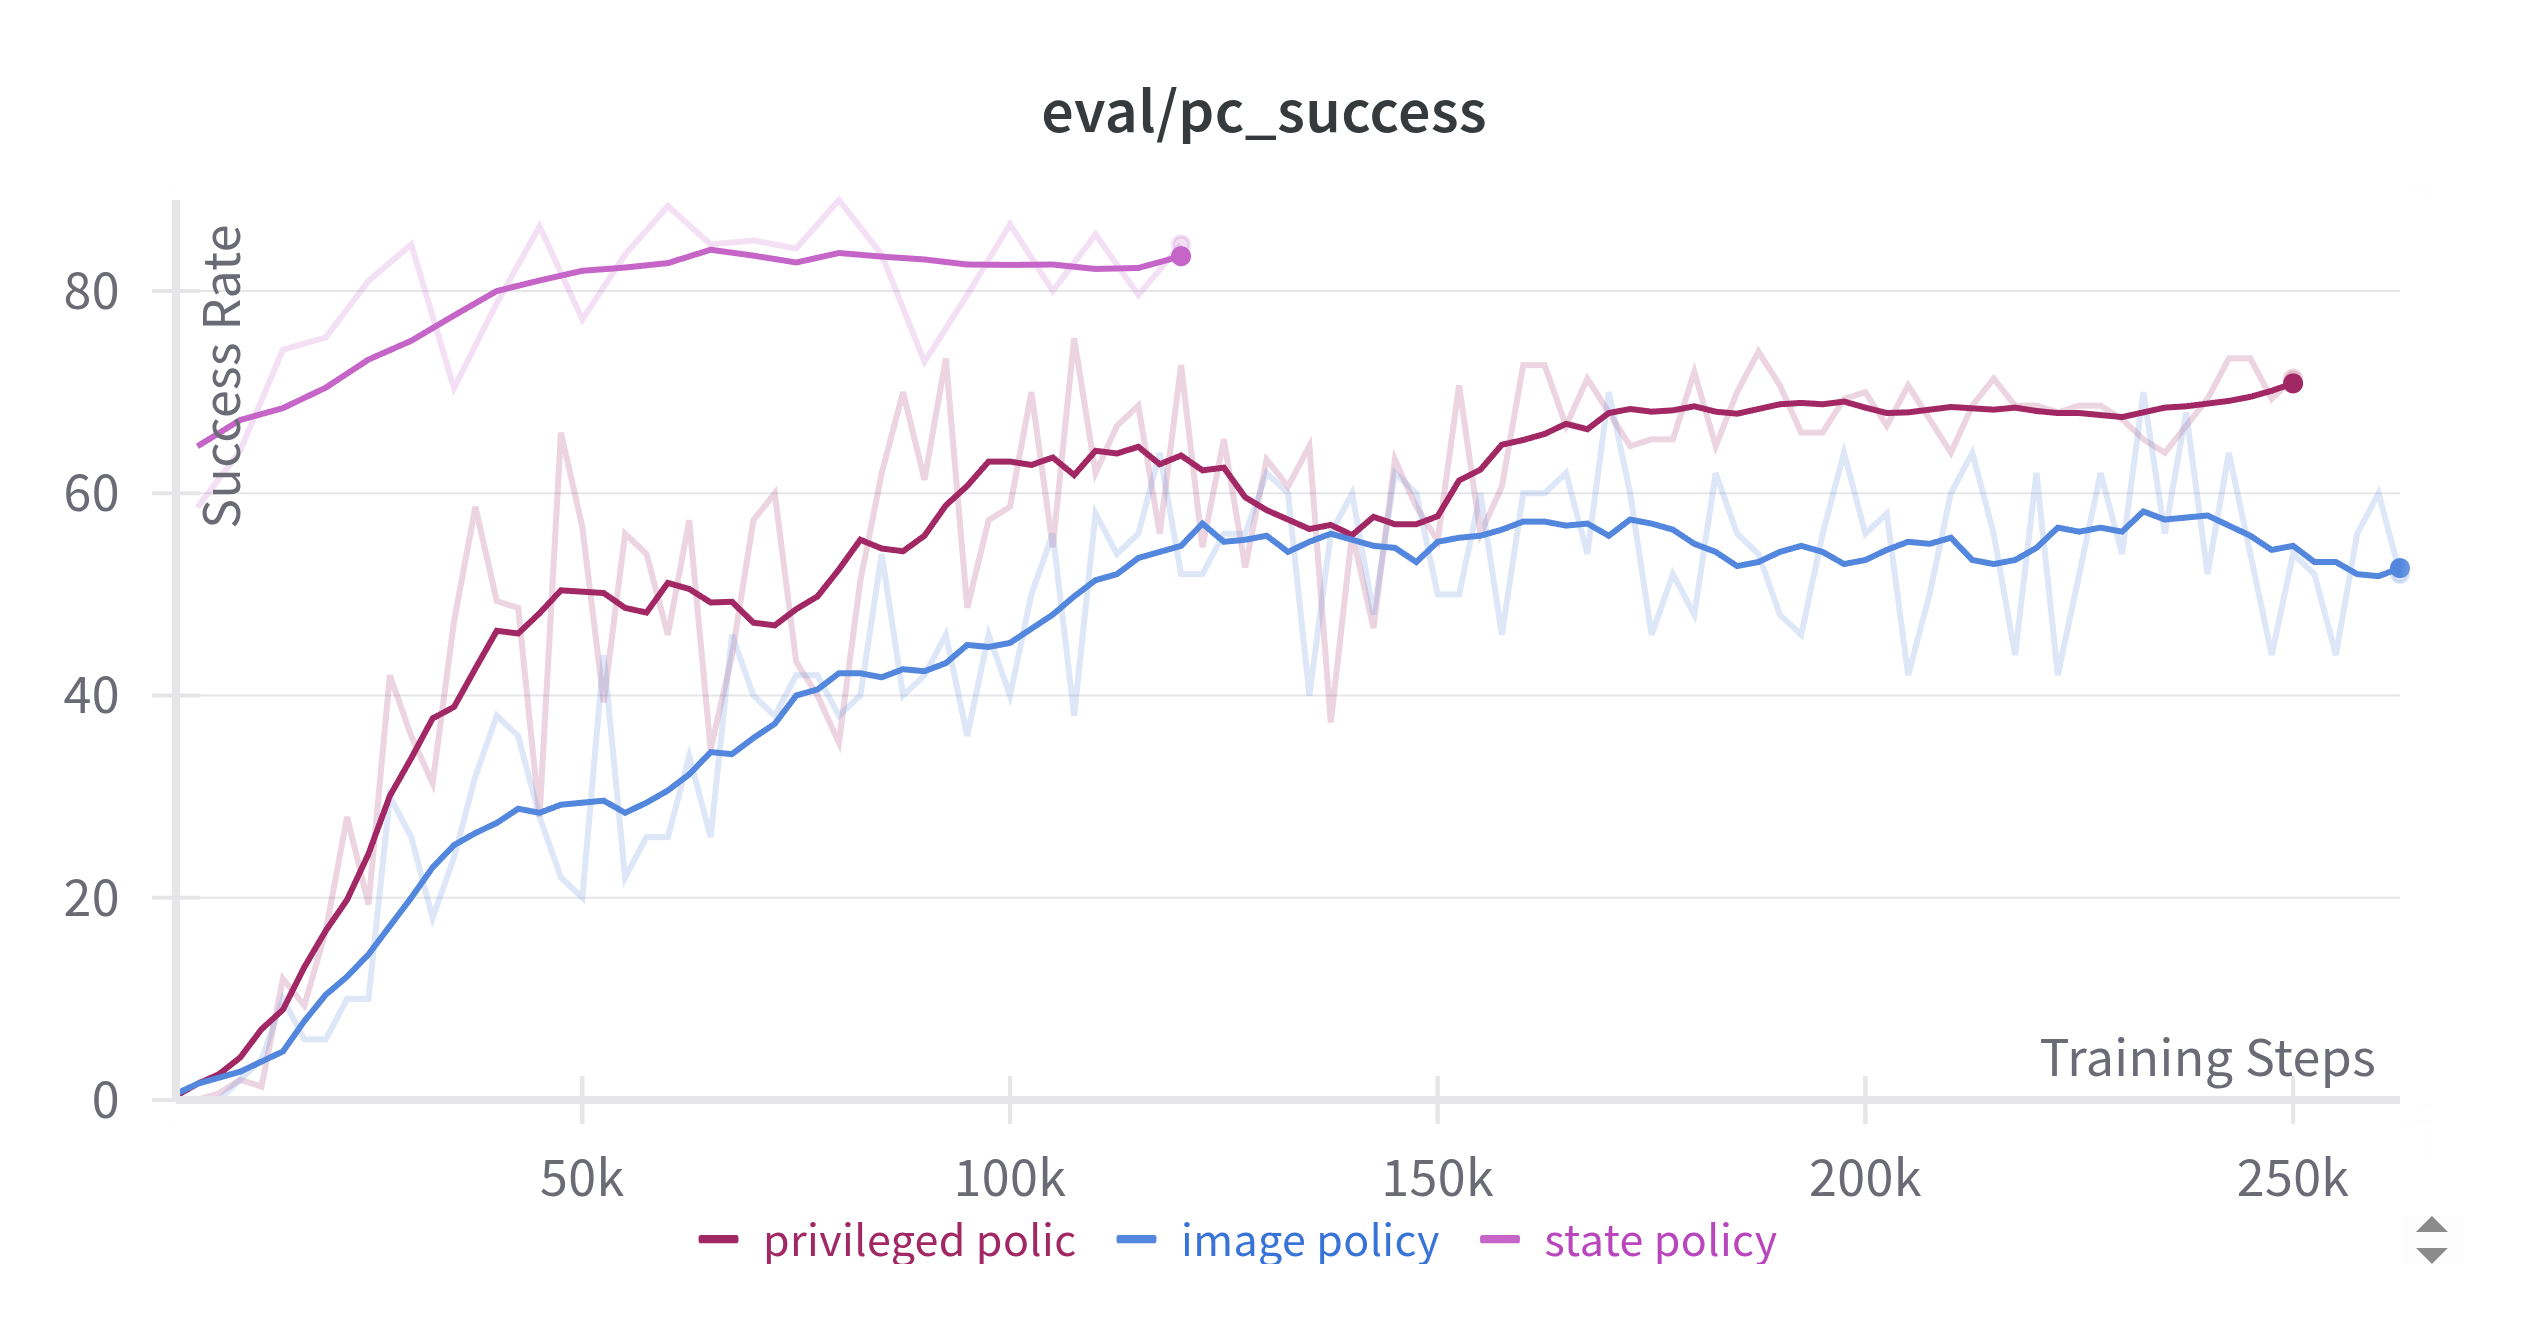
\includegraphics[width=0.8\textwidth]{./media/pushT-privileged-training.png}
    \caption{Performance on the PushT task. The plot shows success rate (y-axis) versus training steps (x-axis) for three policies: a privileged policy using state information directly (pink line, top), an image-based policy trained with access to privileged state information (maroon line, middle), and a baseline state-only policy (blue line, bottom).}
    \label{fig:pusht_performance}
\end{figure}

\labeledparagraph{Baseline Replication - DMFD} We then moved to the SoftGym environment \cite{lin2021softgym}, focusing on the "ClothFold" task, which involves folding a piece of cloth in half with variable initial size, position, and orientation. We reproduced the results from the DMFD paper \cite{salhotra2022learning} and extended them with a sample efficiency study of their framework. This aimed at providing a solid benchmark for a different approach to utilizing privileged information. We conducted a sample efficiency study by training with datasets of varying sizes. The results, reported in Figure \ref{fig:dmfd_clothfold_efficiency}, use the performance metrics defined in Equations \eqref{eq:performance_halftime} and \eqref{eq:norm_performance_halftime}.
To evaluata the sample efficiency differenta training dataset was used, maintaining constant to 8:1 the ratio of demonstrations to variations: including random cloth sizes and initial rotations (\(\pm\pi/4\) radians) of the cloth initialization. 

\begin{figure}[htbp]
    \centering
    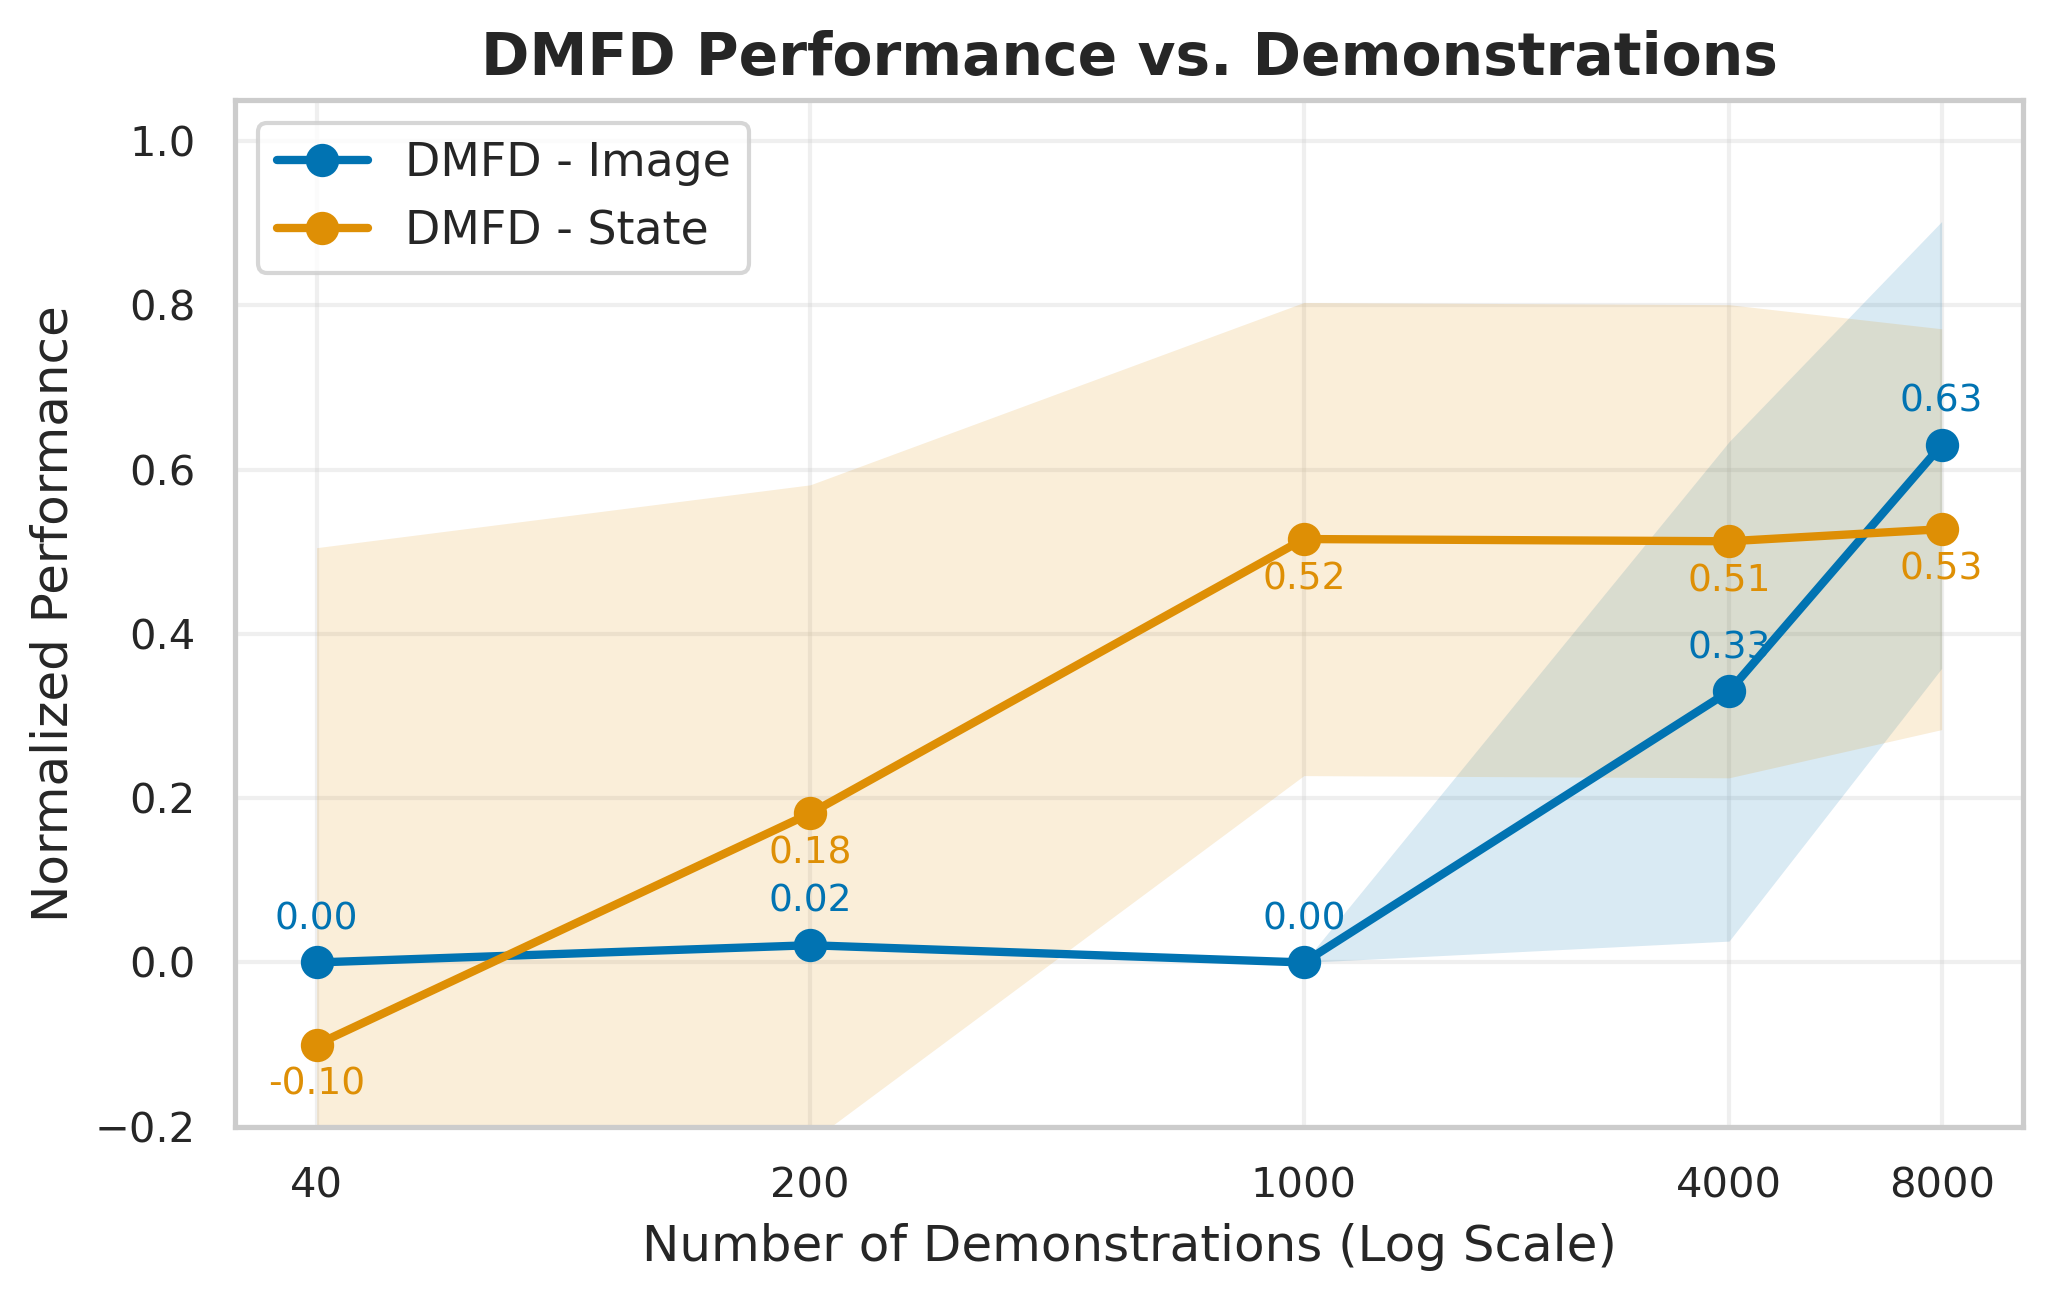
\includegraphics[width=0.7\textwidth]{./media/dmfd-efficiency.png}
    \caption{DMFD Performance vs. Number of Demonstrations on the ClothFold task. The plot shows Normalized Performance (y-axis, higher is better, as defined in Equation~\eqref{eq:norm_performance_halftime}) against the number of training demonstrations (logarithmic x-axis). The DMFD - State policy (orange) generally outperforms the DMFD - Image policy (blue), particularly with fewer demonstrations. Both policies show improved performance with an increasing number of demonstrations. Shaded regions indicate standard deviation. Each data point represents statistics from 100 evaluation episodes (20 episodes across 5 distinct random seeds).}
    \label{fig:dmfd_clothfold_efficiency}
\end{figure}

\labeledparagraph{Behavioral Cloning with Transformer-Based Diffusion Policy on SoftGym's ClothFold Task}
We are currently conducting an experiment to develop policies for the "ClothFold" task in SoftGym \cite{lin2021softgym} using a transformer-based diffusion policy architecture.
Drawing inspiration from Diffusion Policy \cite{chi2023diffusionpolicy}, we employ a behavioral cloning approach.
Our goal is to evaluate the same three policy variants as in the PushT experiments: image-based, state-based, and privileged image-based trained with state features.
Currently, we are particularly focused on developing the "privileged policy" by conducting various experiments to identify the optimal approach for exploiting privileged information.
For instance, we are exploring the integration of a transformer-based shared feature encoder before conditioning the policy, testing different methods for merging information from the image and state pipelines, and evaluating various dropout rates to enhance performance.
Preliminary results from the sample efficiency study of image-based and state-based policies for this approach are presented in Figure \ref{fig:bcdiff_clothfold_efficiency}. The performance metrics align with those defined in Equations \eqref{eq:performance_halftime} and \eqref{eq:norm_performance_halftime}.

\begin{figure}[htbp]
    \centering
    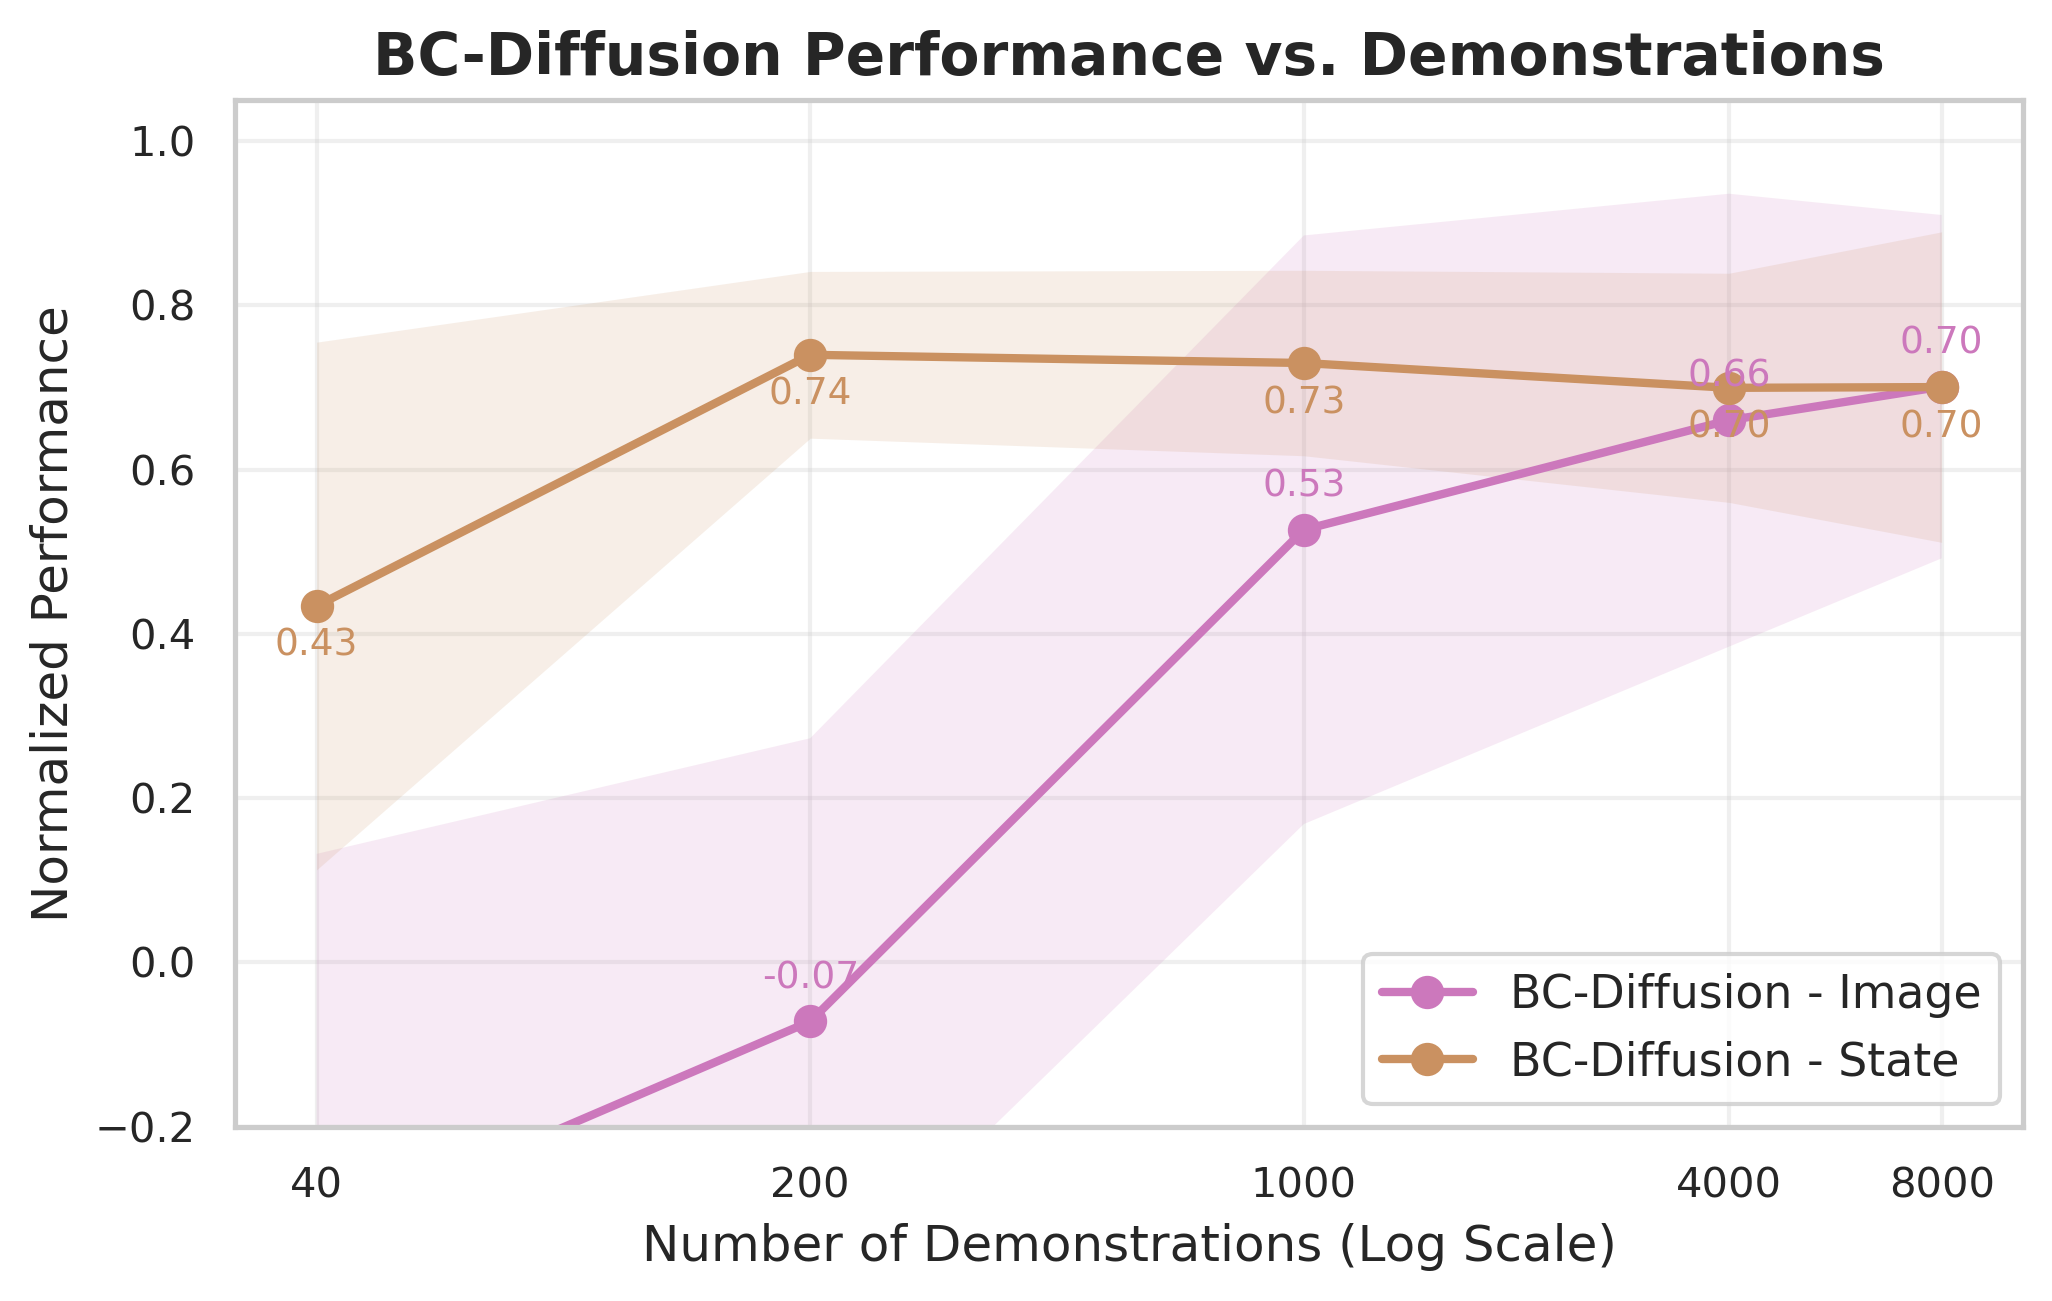
\includegraphics[width=0.7\textwidth]{./media/bc_diffusion_performance_vs_num_dems.png}
    \caption{BC-Diffusion Performance vs. Number of Demonstrations on the ClothFold task. The plot shows Normalized Performance (y-axis, higher is better, as defined in Equation~\eqref{eq:norm_performance_halftime}) against the number of training demonstrations (logarithmic x-axis). Shaded regions indicate standard deviation. Each data point represents statistics from 100 evaluation episodes (20 episodes across 5 distinct random seeds).}
    \label{fig:bcdiff_clothfold_efficiency}
\end{figure}

\newpage

\section*{Future Tests}
Future tests will focus on exploring various strategies to achieve the best results in exploiting privileged information. Some critical tests that we plan to perform include:
\begin{itemize}
    \item Concatenation of inputs combined with dropout to balance the influence of privileged information during training.
    \item Mean Squared Error (MSE) between states and features, inspired by approaches like TrakDis, to align representations.
    \item Contrastive Loss between state and image encoders, similar to techniques used in Rapid Motor Adaptor, to enhance feature correlation.
    \item Expanding on contrastive learning, we will investigate geometric contrastive learning to capture spatial relationships.
    \item Summation of features instead of concatenation to explore alternative methods of information fusion.
\end{itemize}

If satisfactory results are obtained from these experiments, the next step will be to validate our findings on a real-world robot. Executing our experimental results in real-time will significantly strengthen the impact and applicability of our research outcomes.

However, if these tests and additional explorations do not yield the desired performance, we will pivot to an orthogonal approach. This would involve building upon the insights gained and developing a novel framework that leverages a pretrained distribution to achieve sample efficiency in learning.



\section*{Metrics}
\subsection*{ClothFold Task Performance Metrics}
For the ClothFold task, we evaluate performance using two metrics. First, the raw performance \(P\) is calculated based on the particle positions:
\begin{equation} \label{eq:performance_halftime}
P = - \left( \frac{1}{M} \sum_{i \in G_a} \| \mathbf{p}_i - \mathbf{p}_{j(i)} \|_2 \right) - 1.2 \times \left( \frac{1}{M} \sum_{j \in G_b} \| \mathbf{p}_j - \mathbf{p}_{j, init} \|_2 \right)
\end{equation}
where \(M\) is the number of particles per fold group, \(G_a, G_b\) are the particle sets for the two halves being folded together, \(\mathbf{p}_i\) is the current 3D position of particle \(i\), \(\mathbf{p}_{j(i)}\) is the current 3D position of the corresponding particle in the other group, and \(\mathbf{p}_{j, init}\) is the initial 3D position of particle \(j\) in the fixed group.
This raw performance is then normalized to a scale representing the progress from the initial state towards an ideal fold. The ideal performance \(P_{ideal} = 0\) occurs when corresponding particles align (\(\| \mathbf{p}_i - \mathbf{p}_{j(i)} \|_2 \to 0\)) and fixed particles remain stationary (\(\| \mathbf{p}_j - \mathbf{p}_{j, init} \|_2 \to 0\)), causing both terms in Equation~\eqref{eq:performance_halftime} to vanish. The normalized performance is:
\begin{equation} \label{eq:norm_performance_halftime}
P_{\text{norm}} = \frac{P - P_{init}}{P_{ideal} - P_{init}} = \frac{P - P_{init}}{- P_{init}}
\end{equation}
where \(P_{init}\) is the raw performance calculated using Equation~\eqref{eq:performance_halftime} at the start of the episode.


\section*{Targeted Venue}
The targeted venue for publication is the \textbf{International Conference on Intelligent Robots and Systems (IROS)}.

\bibliographystyle{plainnat}
\bibliography{references}

\end{document}
